%!TEX root = ../dissertation.tex
\begin{savequote}[75mm]
Nulla facilisi. In vel sem. Morbi id urna in diam dignissim feugiat. Proin molestie tortor eu velit. Aliquam erat volutpat. Nullam ultrices, diam tempus vulputate egestas, eros pede varius leo.
\qauthor{Quoteauthor Lastname}
\end{savequote}

\chapter{A11Y Tool}
With the successful completion of the A11Y Guide sufficient knowledge had
been gained within the accessibility domain to enable the production of a
tool to identify issues. The fundamental idea behind the tool is to reduce
the feedback loop (and thus the price) of discovering accessibility issues. To
keep the project to a sensible scope the tool will form the "means" by which
accessibility testing could be undertaken but will be limited in the number
of accessibility issues it will identify.

\section{Preparation}
\subsection{Current Process}
The current projects

\subsection{Understanding current solutions}
Prior to building my own I wanted to survey the current landscape of
accessiblity tools. Thanks to the A11Y Guide I had already collected a list of
current testing tools. All but one of the tools target the browser through a
bookmarklet.

\begin{table}[h!]
\centering
\begin{tabular}{ |c|c|c|c| }
 \hline
 Tool & Method & Good & Bad  \\
 \hline
 \hline
 Axe Core & Bookmarklet/Extension &  & a \\
 \hline
 HTML Code Sniffer & Bookmarklet & b & b \\
 \hline
 ESLint JSX A11Y & IDE/CLI & c & c \\
 \hline
 Tota11y & Bookmarklet & d & d \\
 \hline
\end{tabular}
\end{table}

\subsection{What makes this tool different?}


\subsubsection{Browser vs IDE}
Two possible methods for identification of issues

The browser was chosen because


\subsection{Generating ideas}

\subsection{Defining Requirements}

\subsection{Design}
Fig.~\ref{fig:tool_current_design} demonstrates the rough design for most of
the current tools (Tota11y, EsLint). They typically have tightly coupled
components for applying rules and displaying results which limits the way in
which the testing can be done.

\begin{figure}[H]
\centering
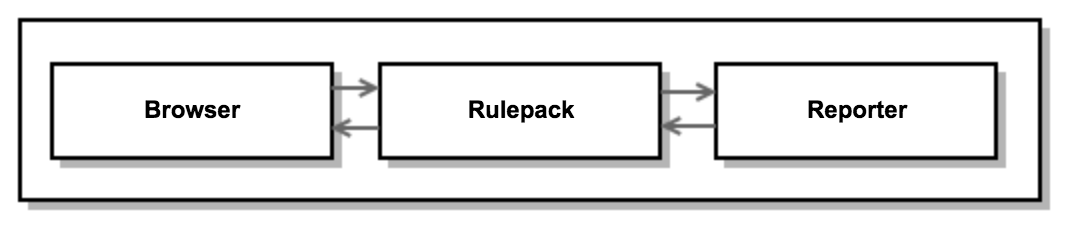
\includegraphics[width=0.8\textwidth]{figures/a11y_tool_current_design}
\captionsetup{justification=centering}
\caption{Current tool design
\label{fig:tool_current_design}}
\end{figure}

% TODO - reference IOC http://www.laputan.org/drc/drc.html
The main limitation in such designs is reusability and customisation. Coming
from a Java background we tend to apply the inversion of control principle to
decouple the reusable components from the specific ones. This comes with the
added benefit of being able to build and test specific modules in isolation.
Fig.~\ref{fig:tool_proposed_design} demonstrates how I propose to apply
this. Components shown in grey demonstrate the possiblites which are opened
by using such a design but are out of scope of this project. The next few
sections in the report will document the design and implementation of each of
the components within scope of the project..

\begin{figure}[H]
\centering
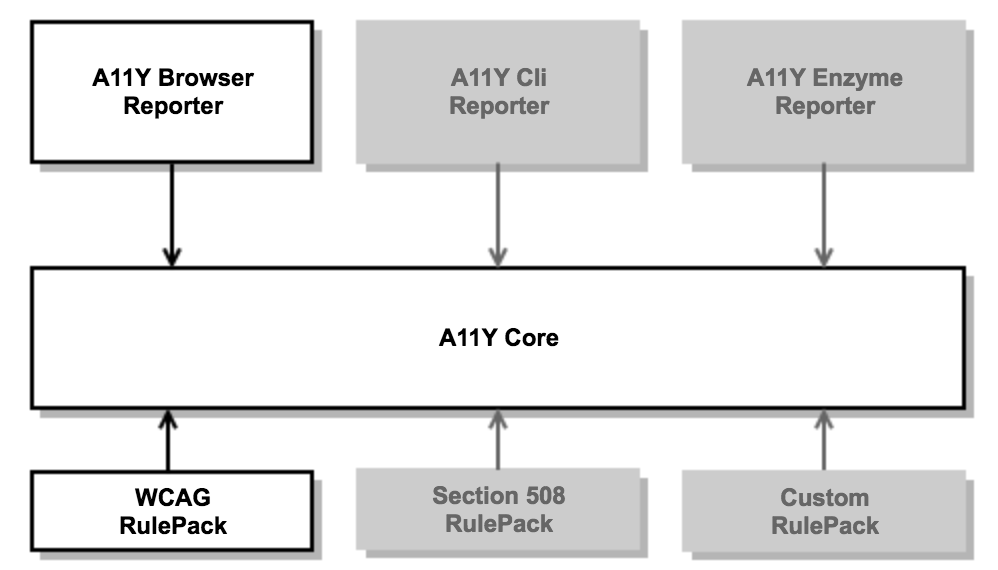
\includegraphics[width=0.7\textwidth]{figures/a11y_tool_proposed_design}
\captionsetup{justification=centering}
\caption{Proposed tool design
\label{fig:tool_proposed_design}}
\end{figure}

\subsubsection{A11Y Core}
This component offers the fundamental building blocks which enable the
others to function. It defines interfaces and common implementations. It is
broken down into a `Checker', `Result' and `Worker'.

%TODO - Reference Semantic Versioning
Due to other components relying upon A11Y Core's interfaces, versioning of
them is important to ensure dependent parties are able to update efficiently.
There are many versioning strategies available and most work on a form of
three digits [major].[minor].[patch]. I always use `Semantic Versioning'
due to the clear definition of when each number should increment. Patch for
bug fixes and non api, Minor for API additions which are backwards compatible
and Major when a breaking API change is introduced. Due to this clarity it is
slowly becoming the defacto standard for software development.

A `Checker' offers a method to check content for issues and give detail
about what they are checking for. Fig.~\ref{fig:checker_design} documents the
initial design for `Checker' and its various implementations.

\begin{figure}[H]
\centering
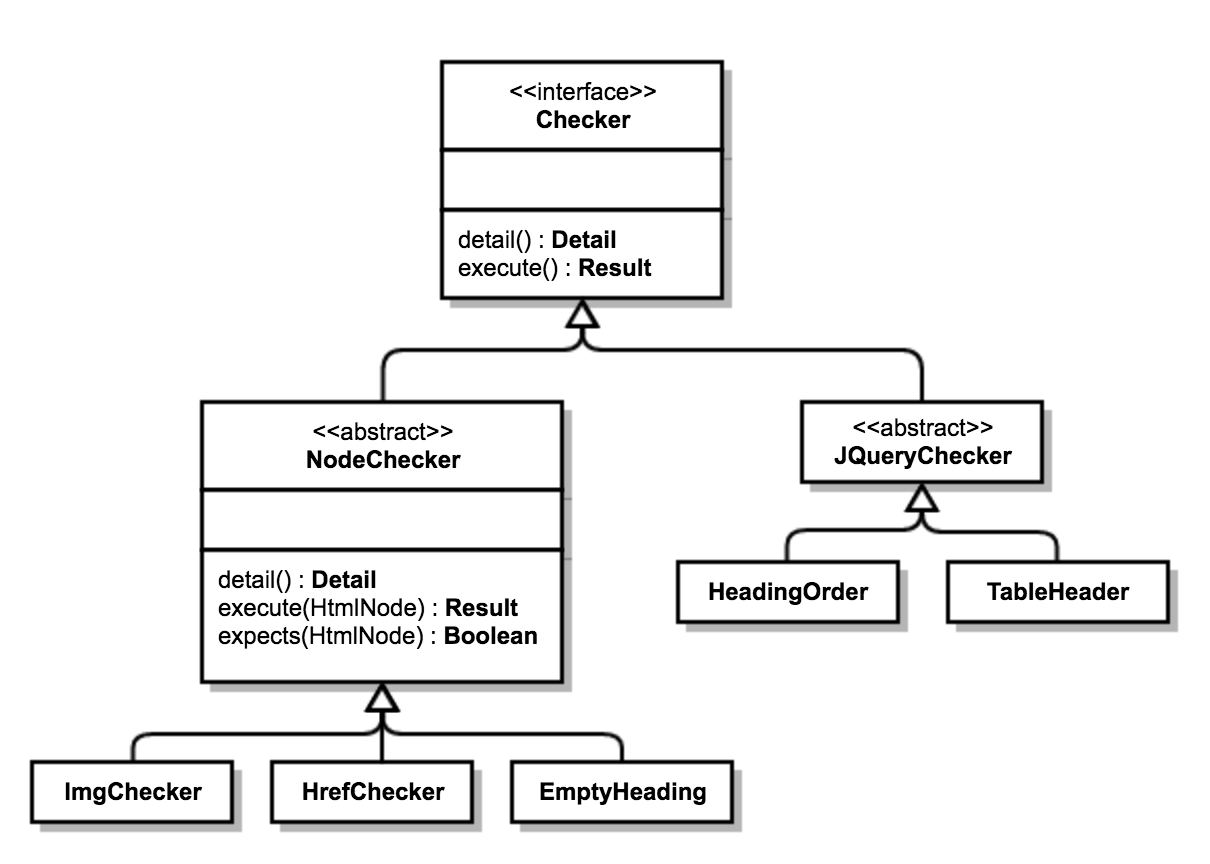
\includegraphics[width=0.6\textwidth]{figures/a11y_tool_checkers}
\captionsetup{justification=centering}
\caption{Proposed `Checker' design
\label{fig:checker_design}}
\end{figure}

Due to EcmaScript's inability to support interfaces I use the constructor to
validate the `instance' for the correct methods at creation time. As these
methods can only exist in child classes it is impossible to create an
instance of `Checker' without them. I felt this was an adequate and efficient
way of creating a framework which others could extend.

\begin{lstlisting}[language=JavaScript]
export default class Checker {
  constructor() {
    this.validateInstance(this.constructor.detail, this.constructor.execute);
  }

  validateInstance(detail, execute) {
    this.validateExists(detail, 'No detail object present');
    this.validateExists(execute, 'No execute method present');
  }

  validateExists(mustExist, error) {
    if(!mustExist) {
      throw new Error(`${this.constructor.name} | ERROR: ` + error);
    }
  }
}
\end{lstlisting}

The `Result' class is an outcome of a `Checker'. They hold the node or element
the `checker' checked and the state either Success, Warn, Info or Error.
Error and Warn have an additional property of
remediation which is to be added by the `Checker' to offer a recommended
method to fix the identified issue. Fig.~\ref{fig:result_design} demonstrates
this structure. It is unlikely that anyone would extend `Result' but similar
to above it has been implemented with interfaces.

\begin{figure}[H]
\centering
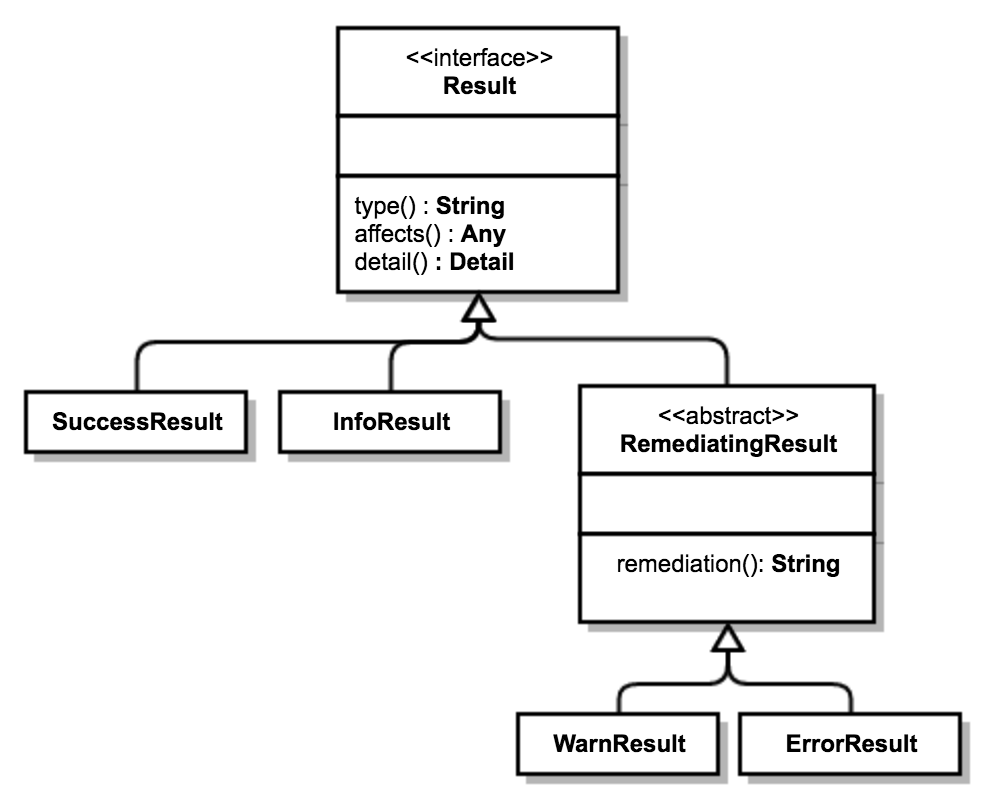
\includegraphics[width=0.6\textwidth]{figures/a11y_tool_result}
\captionsetup{justification=centering}
\caption{Proposed `Result' inheritance structure
\label{fig:result_design}}
\end{figure}

The concept of a `Worker' was added late on during the implementation phase as a
direct result of the performance of `Checker's being poor. Performance issues
were noticeable when iterating around a web pages with a large number of DOM
elements. The worker inverted the for loop and meant that
rather than iterating around the DOM within each `Checker' The DOM was
iterated around only once and each checker was called to perform it's check
only if that DOM node was relevant to it.

`Workers' implement the Singleton Pattern so `Checkers' can be registered from
anywhere. Each individual checker registers itself with it's retrospective
worker. The result of such a design (and the reason this was chosen over others)
is that when a `Checker' is imported into a file it is registered with 'A11Y
Core' and thus available for use. Fig.~\ref{fig:a11y_tool_worker_design}
shows how this works.

\begin{figure}[H]
\centering
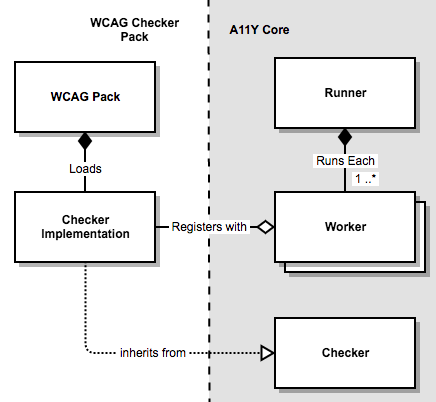
\includegraphics[width=0.5\textwidth]{figures/a11y_tool_worker_design}
\captionsetup{justification=centering}
\caption{Relationships between components and classes
\label{fig:a11y_tool_worker_design}}
\end{figure}

\subsubsection{WCAG Checker Pack}
As shown in Fig.~\ref{fig:a11y_tool_worker_design} above `Checker Packs' are
a collection of `Checkers' loaded into a single file. The requirement for a
'Checker Pack' comes from the fact that the accessibility requirements on
projects change. Some might be required to satisfy the WCAG AA others may
require the Section 508 guidelines.

Below is a snippet from the WCAG 'Checker Pack'. Packs are deliberately easy to
create so users of the tool can create and use their own.

\begin{lstlisting}[language=JavaScript]
import 'checkers/WCAG/HrefChecker.js';
import 'checkers/WCAG/HeadingOrderChecker.js';
import 'checkers/WCAG/TableCaptionChecker.js
\end{lstlisting}

%TODO - Complete this..

\subsubsection{A11Y Browser}
The browser component enables the tool to be ran within a web browser (Tested
on Chrome 57). Fig.~\ref{fig:a11y_tool_browser_design} shows how this fits in
at a high level.

\begin{figure}[H]
\centering
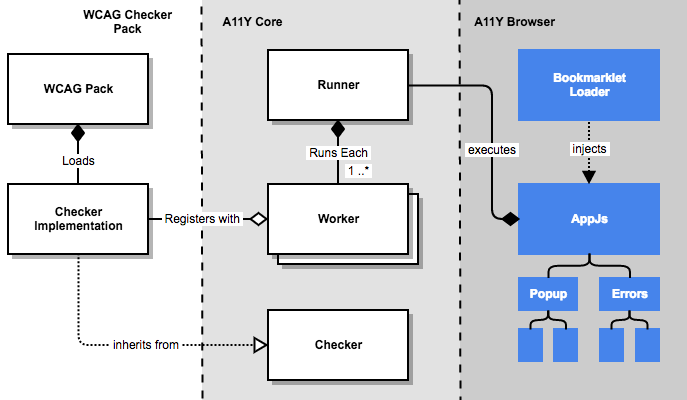
\includegraphics[width=0.75\textwidth]{figures/a11y_tool_browser_design}
\captionsetup{justification=centering}
\caption{How the browser component ties everything together
\label{fig:a11y_tool_browser_design}}
\end{figure}


%\newthought{Lorem ipsum dolor sit amet},
%
%This chapter should describe what was actually produced: the programs which
%were written, the hardware which was built, the theory which was developed or
%the new scientific knowledge acquired.
%
%For software projects, give a high-level overview of your realisation of the
%design. Describe the general organisation of any body of code, web pages,
%database tables, etc, that you have created. Highlight any particularly
%noteworthy aspects, e.g., specialised algorithms, but avoid excessive low-level
%detail. Diagrams and examples are usually valuable.
%
%For research projects, provide a detailed overview of how the research was
%executed (e.g., participants involved, etc). the research results and their
%analysis. Include a description of any statistical analysis methods used.
%Highlight any particularly noteworthy aspects, e.g., especially interesting
%results. Graphs/charts and examples are usually essential. When reporting
%statistical analysis, do not merely present the statistics without interpreting
%their meaning for the reader – e.g., what are the implications of the findings?
%Where applicable, based on the results and analysis, present a set of
%recommendations, guidelines, or itemised list of contributions to knowledge
%that may be derived from your work.
%
%This section should be answering the question: “What did the project actually
%produce?”
